\documentclass[10pt,a4paper,twocolumn]{report}
\usepackage[utf8]{inputenc}
\usepackage[italian]{babel}
\usepackage{amsmath}
\usepackage{amsfonts}
\usepackage{amssymb}
\usepackage{graphicx}
\usepackage{hyperref}
\usepackage{subfig}
\title{Analisi dei clusters}
\begin{document}

\chapter{Analisi dei cluster}
\section{clustering via K-means}
\subsection{Scelta degli attributi e della funzione distanza}
% scelta delle features
Si sono scelti gli attributi quantitativi ($satisfaction\_level$, $last\_evaluation$, $average\_montly\_hours$, $time\_spend\_company$) e l'attributo numerico ordinale $number\_project$. 
La scelta degli attributi quantitivi è giustificata dal fatto che l'algoritmo K-means richiede di calcolare la media, la quale è definita solo per gli attributi quantitiativi. 
L'unica eccezione è stata fatta per l'attributo $number\_project$ essendo oridinale.
L'interpretazione è stata che se $number\_project$ ha valore frazionario $d.f$ (con $d$ parte intera, $f$ parte float) per un dato centroide, allora il cluster da lui rappresentato contiene gli impiegati che in media hanno fatto tra $d$ e $d+1$ progetti.
% scelta della funzione distanza
\paragraph{}
La funzione distanza scelta è stata la distanza Euclidea perché i centroidi sono medie nello spazio Euclideo in $\Re^{n}$, dove $n$ è il numero di attributi. [TODO: spiega meglio]

\subsection{Identificazione del miglior valore di k}
Identificare il numero di clusters è importante per trovare un compromesso tra pochi grandi clusters e molti piccoli, e spesso insignificanti, clusters. Per indentificare il miglior valore di $k$ per l'algoritmo K-means si è monitorato l'andamento della $Sum\ of\ Squared\ Error\ (SSE)$ e la $silhouette\ score$ al variare di $k$, il cui grafico è riportato in \autoref{fig:sse_sil_vs_k}. Il grafico della $SSE$ ha un andamento non-crescente e diminuisce in maniera smooth, mentre la silhouette presenta molti picchi.

\begin{figure}[hbtp]
\centering
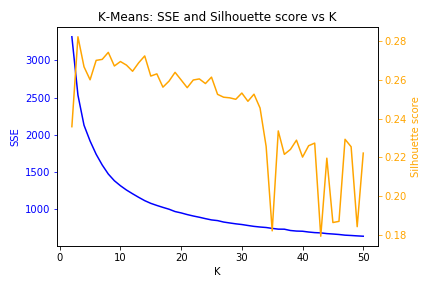
\includegraphics[width=1\columnwidth]{../images/sse_silhouette_vs_k.png}
\caption{Andamento della SSE e silhouette al variare di k. Il punto di gomito è scelto per $k=8$, cui corrisponde $SSE=1474$ e $silhouette=0.27$.}
\label{fig:sse_sil_vs_k}
\end{figure}%

% scelta del punto di gomito
\paragraph{}
Sucessivamente si è scelto il punto di gomito della $SSE$ combinando un approccio visivo ad uno quantitativo, analizzando i punti $k$ in cui era presente un maggior calo di $SSE$. La scelta finale per il valore di $k$ ha preso in considerazione anche il corrispondente valore della $silhouette$. La $silhouette$ assumeva valori nel range $\left[0.18, 0.28\right]$ con minimo per $k=47$ e massimo per $k=3$, mentre la $SSE$ assumeva valori tra $\left[640, 3315\right]$ con minimo per $k=50$ e massimo per $k=2$. Inoltre, sono stati presi in considerazione i top 10 valori di $k$ corrispondenti a un maggiore calo della $SSE$ ($top\_diffs$), e, analogamente i top 10 $k$ con maggiore $silhouette$ ($top\_silho$). Si sono ottenuti i seguenti insiemi di valori di $k$, candidati ad essere punti di gomito: $top\_diffs=\lbrace3,4,5,6,7,8,9,10,11,12\rbrace$ and $top\_silho\lbrace3,8,14,7,6,10,5,9,4,18\rbrace$. Mettendo insieme tutte le precendenti informazioni e considerando l'insieme $top\_diffs \cap top\_silho$, si è scelto il punto di gomito $k=8$, corrispondente a $SSE=1474$ and $silhouette=0.27$.

\paragraph{}
Alternativamente, scegliendo il punto del grafico della $SSE$ più vicino all'origine in norma Euclidea, si era ottenuto il punto $k=12$, con $SSE=1210$ e $silhouette=0.27$.

\subsection{Caratterizzazione dei clusters ottenuti}
La caratterizzazione dei cluster ottenuti è stata svolta per mezzo dell'analisi dei centroidi, e confrontando le distribuzioni degli attributi dei singoli cluster con quelle dell'intero dataset.
% analisi per centroidi
\paragraph{}
La \autoref{fig:centroids} riporta l'analisi per centroidi. Gli attributi dei centroidi dei clusters 1 e 3 hanno relativamente lo stesso andamento. In particolare i valori di $average\_montly\_hours$ differiscono di poco. Questo significa che per valori più piccoli di $k$ i due clusters potrebbero unirsi. I clusters 4, 5 e 7 sono caratterizzati da un basso valore di $satisfaction\_level$, mentre lo stesso attributo assume valori elevati nei clusters 0, 1, 3 e 6. Il cluster 6 è l'unico con un alto valore di $time\_spend\_company$, mentre per il resto dei clusters l'attributo assume valori bassi. Questo ci dice che i due attributi non sono correlati, altrimenti anche i clusters 0, 1 e 3 avrebbero avuto un alto valore di $time\_spend\_company$. Il cluster 4 ha il più basso valore di $satisfaction\_level$ e il più alto valore di  $average\_montly\_hours$. Inoltre, il cluster 4 ha il più alto valore di $number\_projects$ e un relativamente basso valore di $time\_spend\_company$. Questo significa che il sovraccarico di lavoro dovuto ad una grande quantità di progetti, svolti in poco tempo, porta gli impiegati ad essere infelici.

\begin{figure}[hbtp]
\centering
\textbf{analisi dei k centroidi}\par
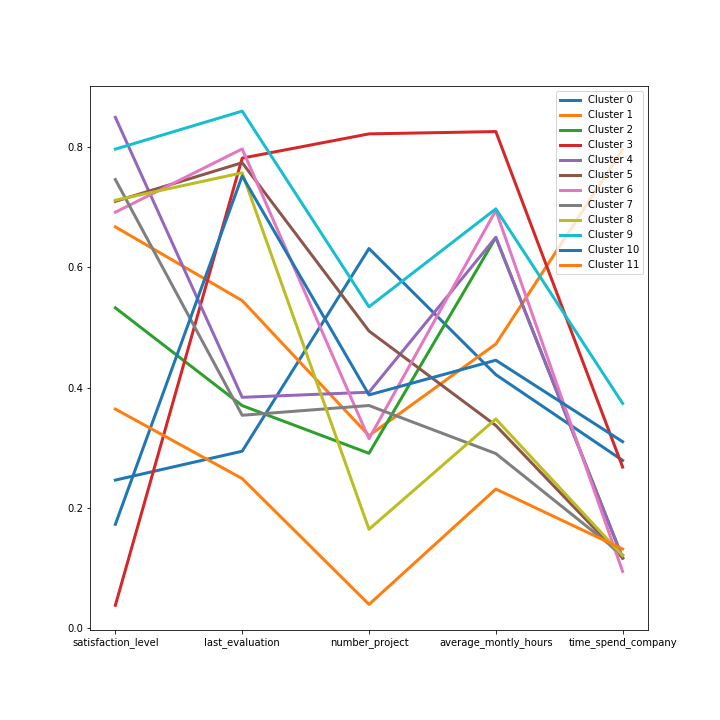
\includegraphics[width=1\columnwidth]{../images/k-centroids_analysis.png}
\caption{Analisi dei valori degli attributi dei centroidi ottenuti. Ogni centroide è rappresentato da un insieme di segmenti, i cui estremi marcano i valori degli attributi. Gli attributi dei clusters 1 e 3 seguono lo stesso andamento.}
\label{fig:centroids}
\end{figure}

% confronto delle distribuzioni degli attributi
\paragraph{}
In \autoref{fig:kde_clusters} viene fatto un confronto tra le distribuzioni degli attributi dell'intero dataset e quelle dei singoli clusters, in particolare i cluster 4 e 7. L'attributo $number\_project$ assume una distribuizione multi-modale per tutte le kernel density estimation, essendo un attributo intero. Gli attributi $last\_evaluation$ e $average\_montly\_hours$ hanno una distribuzione simile alla normale, ma leggermente schiacciata. Gli stessi attributi assumono una simile forma per il cluster 4. Invece per l'intero dataset i due attributi hanno una distribuzione bi-modale con picchi poco pronunciati, divisi da un lungo plateau. In entrambe le figure \ref{fig:kde_4} e \ref{fig:kde_7} è presente un picco molto acuto per l'attributo $satisfaction\_level$. Entrambi i picchi sono quasi simmetrici, se non per lo scalino nella parte finale a destra del punto medio. Questo comportamento non è ripetuto per l'intero dataset. L'attributo $time\_spend\_company$ assume una distribuzione multi-modale per il cluster 7, con 5 picchi nell'intervallo $\left[0, 0.5\right]$. 
Mentre per il cluster 4, 
$time\_spend\_company$ ha meno variabilità riportando un picco relativamente acuto centrato in $0.25$, e altri due picchi meno pronunciati.

\begin{figure*}%
    \centering
    \subfloat[]
    {
    	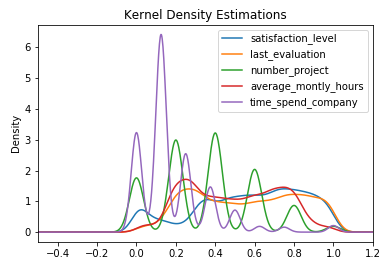
\includegraphics[width=0.3\textwidth]{../images/kde_quantitative_features.png}
    	\label{fig:kde_dataset}
    }%
    %\qquad
    \subfloat[]
    {
    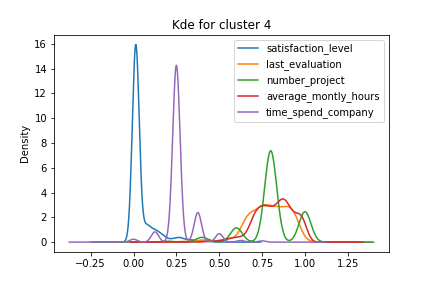
\includegraphics[width=0.3\textwidth]{../images/kde_within_clusters_c4.png}
    \label{fig:kde_4}
    }%
    %\qquad
    \subfloat[]
    {
    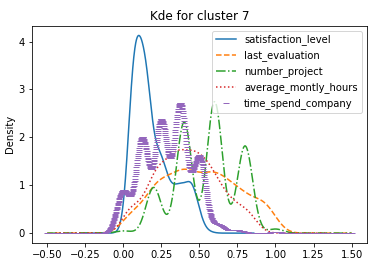
\includegraphics[width=0.3\textwidth]{../images/kde_within_clusters_c7.png}
    \label{fig:kde_7}
    }%
    \caption{Kernel density estimation degli attributi 
    		\protect\subref{fig:kde_dataset} per l'intero dataset, 
    		\protect\subref{fig:kde_4} per il cluster 4, e
    		\protect\subref{fig:kde_7} per il cluster 7. Gli acuti picchi dell'attributo $satisfaction\_level$ per i cluster 4 e 7 non sono così pronunciati anche nell'intero dataset.}%
    \label{fig:kde_clusters}%
\end{figure*}

\subsection{Visualizzazione del clustering via Principal Component Analysis}
I risultati ottenuti dal clustering via K-means sono stati combinati con la PCA per visualizzare la proiezione di ogni punto di dati in due dimensioni. Il dataset ha una forma globulare allungata, simile ad un ellisse. I punti di dati sono molto vicini gli uni agli altri formando un dataset molto denso, in cui i cluster 4 e 5 sono molto definiti, mentre i punti degli altri clusters tendono a mischiarsi. In basso a sinistra è presente una zona di bassa densità di punti appartenenti al cluster 0, mentre in alto a destra vi è un chiaro outlier assegnato al cluster 7. La natura dell'outlier in termini di attributi non è stata approfondita.

\begin{figure}[hbtp]
\centering 
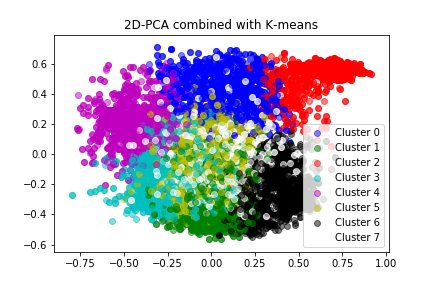
\includegraphics[width=1\columnwidth]{../images/pca_kmeans.png}
\caption{visualizzazione del clustering in 2D. Ad ogni punto di dati è associata una label. Ogni label è rappresentata con un colore. Dataset denso a forma di ellisse. Un outlier è chiaramente presente in alto a destra.}
\label{fig:pca_kmeans}
\end{figure}

\section{Clustering via DBSCAN}


\end{document}